\documentclass[10pt,a4paper]{article}

% Language setting
% Replace `english' with e.g. `spanish' to change the document language
\usepackage[utf8]{inputenc}
%\usepackage[latin1]{inputenc}

% Set page size and margins
% Replace `letterpaper' with`a4paper' for UK/EU standard size
\usepackage[letterpaper,top=2cm,bottom=2cm,left=3cm,right=3cm,marginparwidth=1.75cm]{geometry}

% Useful packages
\usepackage{amsmath}
\usepackage{graphicx}
\usepackage[colorlinks=true, allcolors=blue]{hyperref}
\usepackage{float}
\usepackage{listings}
\usepackage{color}
\usepackage{listingsutf8}
\usepackage{enumitem}
\usepackage[demo]{graphicx}
\usepackage{subfig}

\definecolor{dkgreen}{rgb}{0,0.6,0}
\definecolor{gray}{rgb}{0.5,0.5,0.5}
\definecolor{mauve}{rgb}{0.58,0,0.82}

\lstset{frame=tb,
  language=Java,
  aboveskip=3mm,
  belowskip=3mm,
  showstringspaces=false,
  columns=flexible,
  basicstyle={\small\ttfamily},
  numbers=none,
  numberstyle=\tiny\color{gray},
  keywordstyle=\color{blue},
  commentstyle=\color{dkgreen},
  stringstyle=\color{mauve},
  breaklines=true,
  breakatwhitespace=true,
  tabsize=3,
  % https://en.wikibooks.org/wiki/LaTeX/Special_Characters
  literate=%
    {ã}{\~{a}}1
    {à}{\`{a}}1
    {á}{\'{a}}1
    {â}{\^{a}}1
    {é}{\'{e}}1
    {ê}{\^{e}}1
    {í}{\'{i}}1
    {õ}{\~{o}}1
    {ò}{\`{o}}1
    {ó}{\'{o}}1
    {ô}{\^{o}}1
    {ú}{\'{u}}1
    {ç}{\c{c}}1
    {Σ}{\\Sigma}1
}

\title{Documentação de atividades do Grupo 5 \\ Processamento de Imagens Digitais \\ Professor Leandro Alves Neves}
\author{Anderson Garrido Scaioni (anderson.garrido@unesp.br) \\ Andréia Salmazo Bertasso (andreia.bertasso2@etec.sp.gov.br) \\ Johny William de Oliveira Alves (johnywalves@gmail.com)}

\begin{document}
\maketitle

\begin{flushleft}
\textbf{Uso pacotes e criação da biblioteca}
\end{flushleft}

\begin{flushleft}
Foram instaladas os pacotes do Python Package Index (PyPI), um repositório de software para a linguagem de programação Python, fazendo uso do comando
\end{flushleft}

\begin{lstlisting}[language=Bash]
pip install pillow matplotlib scikit-learn
\end{lstlisting}

\begin{flushleft}
Para facilitar a apresentação dos resultados posteriores e algumas rotinas foram usadas algumas funções reutilizadas
\end{flushleft}

\lstinputlisting[language=Python]{sources/library.py}

\pagebreak

\section{Criação e Rotulagem de Imagens - Exercício 6}

\subsection{Enunciado}

Escreva um programa para reproduzir as imagens apresentadas no slide 41. Considere que as imagens têm dimensões: 256x256 com 256 níveis de profundidade. Em seguida, o programa deve ser capaz de apresentar a taxa de amostragem e a profundidade de cada imagem.

\subsection{Código Fonte}

\lstinputlisting[language=Python]{sources/01_generate_images.py}

\subsection{Explicação}

\begin{flushleft}
O programa para geração de imagens foi criado na linguagem Python e utiliza o pacote “Pillow”, foi definida a função {\ttfamily create\textunderscore images(name, quantization)} que cria a imagem com os parâmetros name (nome da imagem) e quantization (quantificação dos cinzas), nessa função {\ttfamily img = Image.new('P', (256, 256))} a imagem criada é de 8 bits de profundidade com tamanho 256x256 pixels, após a geração da imagem ela é salva em disco na pasta images com a extensão bmp conforme o seguinte código  {\ttfamily  img.save('./images/' + name + '.bmp')}.
\end{flushleft}

\begin{flushleft}
A função é executada 5 vezes, para gerar assim as imagens a.bmp, b.bmp, c.bmp, d.bmp e e.bmp na pasta images.  
\end{flushleft}

\begin{figure}[H]
    \centering
    \subfloat[\centering a.bmp]{{
\includegraphics[width=2cm]{images_generate/01/a.jpg}}}%
    \qquad
    \subfloat[\centering b.bmp]{{
\includegraphics[width=2cm]{images_generate/01/b.jpg}}}%
    \qquad
    \subfloat[\centering c.bmp]{{
\includegraphics[width=2cm]{images_generate/01/c.jpg}}}%
    \qquad
    \subfloat[\centering d.bmp]{{
\includegraphics[width=2cm]{images_generate/01/d.jpg}}}%
    \qquad
    \subfloat[\centering e.bmp]{{
\includegraphics[width=2cm]{images_generate/01/e.jpg}}}%
\end{figure}

\pagebreak

\section{Criação e Rotulagem de Imagens - Exercício 11}

\subsection{Enunciado}

\begin{flushleft}
Considere as imagens produzidas no Exercício 6 e implemente um programa para realizar a rotulagem de componentes conexos (cluster/aglomerado). A rotulagem deve ser realizada por meio do “Hoshen–Kopelman algorithm”. O programa deve fornecer o total de componentes conexos e os rótulos atribuídos em cada região da imagem dada como entrada. Use vizinhança-8 como critério. Por fim, considerando a imagem (e) após a rotulagem, o programa deve apresentar as distâncias (D\textsubscript{e}, D\textsubscript{4} e D\textsubscript{8}) entre os centros de dois componentes conexos (definidos (sorteados) aleatoriamente).
\end{flushleft}

\subsection{Código Fonte}

\lstinputlisting[language=Python]{sources/02_clustering_images.py}

\subsection{Explicação}

\begin{flushleft}
A implementação do algortimo para clursterização tem como base o algoritmo de rotulagem "Hoshen-Kopelman", adaptado para utilizar vizinhaça 8 e agrupar pela quantização de cinza, a linguagem de programação é Python juntamente com o pacote "Pillow".
\end{flushleft}

\begin{flushleft}
Definido o número de linhas e colunas (256x256) vindo das imagens e um vetor com as possíveis cores a rotulagem.
\end{flushleft}

\begin{flushleft}
Três funções para calcular a distância foram implementadas:
\end{flushleft}

\begin{itemize}
    \item {\ttfamily distance\textunderscore euclidean(first, second)};
    \item {\ttfamily distance\textunderscore four(first, second)};
    \item {\ttfamily distance\textunderscore eight(first, second)}.
\end{itemize}

\begin{flushleft}
A função {\ttfamily cluster\textunderscore image(name)} realiza a rotulagem através de cores e quando executada utiliza as funções:
\end{flushleft}

\begin{itemize}
   \item {\ttfamily find(labels, x)};
   \item {\ttfamily union(labels, x, y)}.
 \end{itemize}

\begin{flushleft}
A imagem clursterizada é salva na pasta "images" com o nome da imagem original adicionado de "\textunderscore clustered.bmp", após a imagem ser salva é exibido nome da imagem original, quantidade de grupos e rótulos dos grupos. 
\end{flushleft}

\begin{flushleft}
Se a imagem a ser clursterizada for a imagem "e.bmp" é calculada as distância euclidiana, distância quatro (\textit{city-block}) e distância oito (\textit{chessboard}) de dois aglomerados conexos, selecionados aleatoriamente e verificados pela função {\ttfamily is\textunderscore connected(first, second)}
\end{flushleft}

\begin{flushleft}
A função {\ttfamily cluster\textunderscore image} é executada 5 vezes uma para cada imagem gerada no exercício anterior.
\end{flushleft}

\lstinputlisting[language=Bash]{outputs/02_clustering_images.txt}

\begin{flushleft}
Assim também temos as imagens cluterizadas
\end{flushleft}

\begin{figure}[H]
    \centering
    \subfloat[\centering a.bmp]{{
\includegraphics[width=2cm]{images_generate/02/a_clustered.jpg}}}%
    \qquad
    \subfloat[\centering b.bmp]{{
\includegraphics[width=2cm]{images_generate/02/b_clustered.jpg}}}%
    \qquad
    \subfloat[\centering c.bmp]{{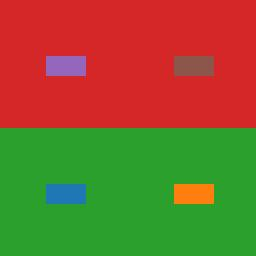
\includegraphics[width=2cm]{images_generate/02/c_clustered.jpg}}}%
    \qquad
    \subfloat[\centering d.bmp]{{
\includegraphics[width=2cm]{images_generate/02/d_clustered.jpg}}}%
    \qquad
    \subfloat[\centering e.bmp]{{
\includegraphics[width=2cm]{images_generate/02/e_clustered.jpg}}}%
\end{figure}

\pagebreak

\section{Ruído - Exercício 4}

\subsection{Enunciado}

Dada a imagem (e) com e sem a presença de ruído gaussiano (exercício 3), compare-as por meio das métricas  \textit{erro máximo}, \textit{erro médio absoluto}, \textit{erro médio quadrático}, \textit{raiz do erro médio quadrático}, \textit{erro médio quadrático normalizado} e \textit{coeficiente de Jaccard} para identificar os níveis de similaridades existentes.

\begin{enumerate}[label=\roman*.]
    \item Observando os valores obtidos, é possível definir algum comportamento padrão entre as métricas a partir dos ruídos aplicados em cada imagem?
    \item Neste cenário, qual métrica permite evidenciar melhor a degradação da imagem em razão da presença de ruído? Justifique sua resposta.
\end{enumerate}

\subsection{Código Fonte}

\lstinputlisting[language=Python]{sources/03_noise_gaussian.py}

\subsection{Saída}

\lstinputlisting[language=Bash]{outputs/03_noise_gaussian.txt}

\subsection{Conclusão}

\begin{enumerate}[label=\roman*.]
\item Observando os valores obtidos, é possível definir um padrão de picos inversamente proporcional ao histograma da imagem original de forma que o coeficiente de Jacard indica similidade entre as duas imagens, mostra bem a deterioração do conteúdo original

\begin{figure}[H]
    \centering
    \subfloat[\centering Imagem original]{{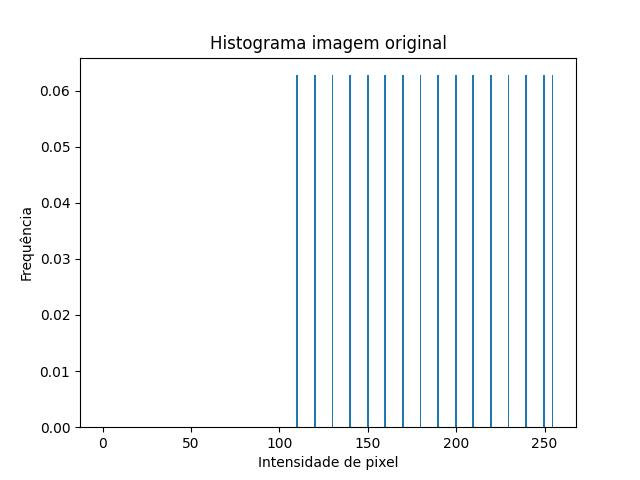
\includegraphics[width=4.5cm]{images_generate/03/e_histogram.jpg}}}%
    \qquad
    \subfloat[\centering Ruído gaussiano]{{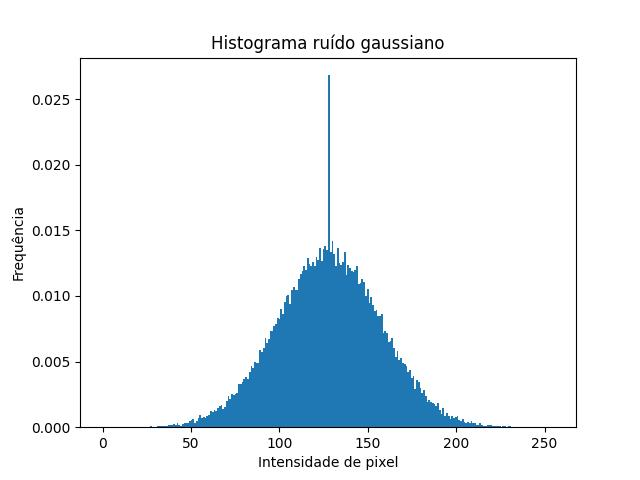
\includegraphics[width=4.5cm]{images_generate/03/noise_histogram.jpg}}}%
    \qquad
    \subfloat[\centering Imagem ruidosa]{{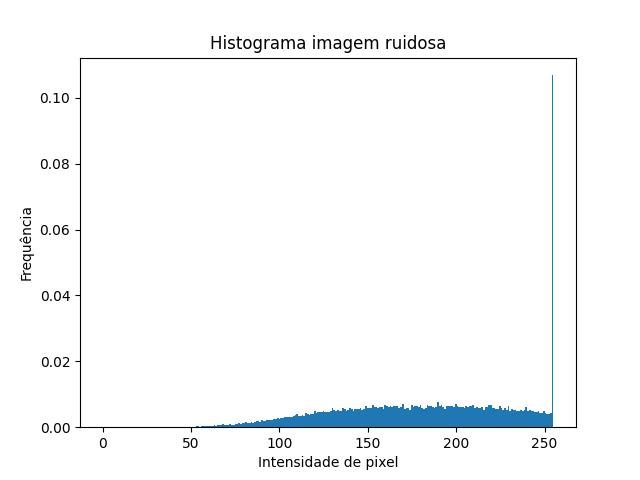
\includegraphics[width=4.5cm]{images_generate/03/e_noised_histogram.jpg}}}%
\end{figure}

\item O erro médio quadrático com resultado 94.27720642089844 para o desvio padrão de 30 por possuir uma variância maior sobre os outros valores que permite evidenciar melhor a degradação da imagem em razão da presença de ruído, evidenciado pela figura e\textunderscore noise\textunderscore gaussian.bmp apresentado abaixo

\begin{figure}[H]
    \centering
    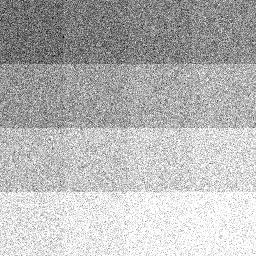
\includegraphics[scale=0.9]{images_generate/03/e_noise_gaussian.jpg}
    \caption{Figura e\textunderscore noise\textunderscore gaussian.bmp}
    \label{fig:enoisegausian}
\end{figure}

\end{enumerate}

\pagebreak

\section{Ruído - Exercício 5}

\subsection{Enunciado}

Descreva cada etapa para ilustrar o processo de aplicação de ruídos em uma imagem A (5x5), com níveis de cinza definidos aleatoriamente. Para tanto, determine os parâmetros
iniciais para produzir uma imagem B (representativa do ruído em questão) e, em seguida, apresente: 

\begin{enumerate}[label=\alph*.]
   \item o resultado da função p(z);
   \item a imagem B representativa do ruído;
   \item o histograma de B para mostrar a característica do ruído;
   \item a matriz A após ser degrada por B;
   \item o histograma do resultado obtido em (d).
\end{enumerate}

 Esses experimentos devem ser realizados com os ruídos gaussiano e poisson (shot noise) ou salt-and-pepper noise.

\subsection{Código Fonte}

\lstinputlisting[language=Python]{sources/04_noise_gaussian_poisson.py}

\subsection{Saída}

\lstinputlisting[language=Bash]{outputs/04_noise_gaussian_poisson.txt}

\begin{figure}[H]
    \centering
    \subfloat[\centering Função p(z) do ruído de Gaussiano]{{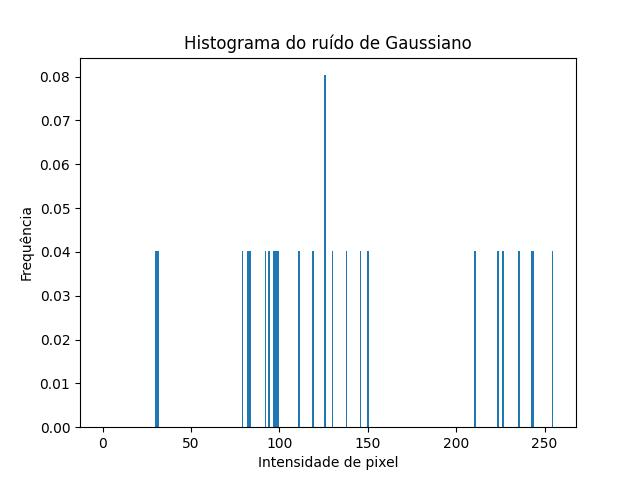
\includegraphics[width=6cm]{images_generate/04/pz_gauss_degraded.jpg}}}%
    \qquad
    \subfloat[\centering Histograma do ruído de Gaussiano]{{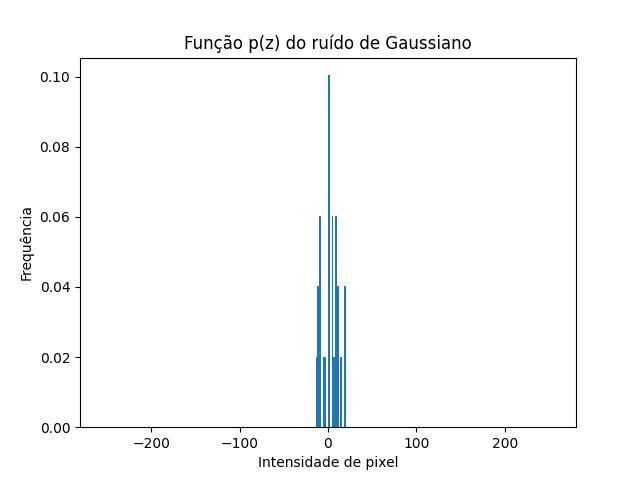
\includegraphics[width=6cm]{images_generate/04/pz_gauss_noise.jpg}}}%
    \qquad
    \centering
    \subfloat[\centering Função p(z) do ruído Poisson]{{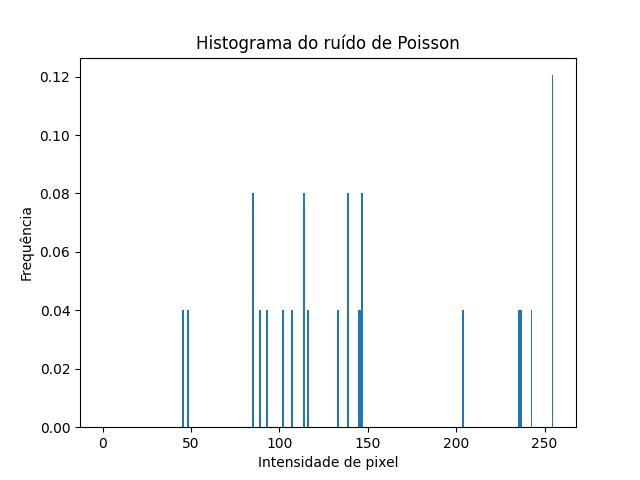
\includegraphics[width=6cm]{images_generate/04/pz_poisson_degraded.jpg}}}%
    \qquad
    \subfloat[\centering Histograma do ruído de Poison]{{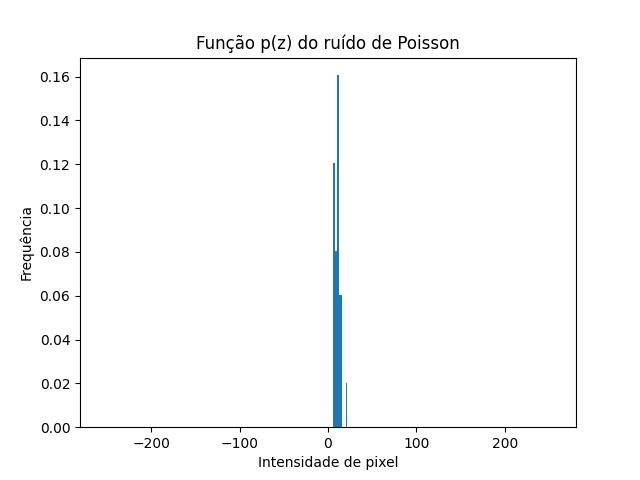
\includegraphics[width=6cm]{images_generate/04/pz_poisson_noise.jpg}}}%
    \qquad
\end{figure}

\subsection{Explicação}

\begin{flushleft}
1. Para resolução dessa questão devemos  Importar as bibliotecas necessárias para trabalhar na linguagem Python e também utlizamos uma biblioteca própria descrita no início do documento.
\end{flushleft}

\begin{lstlisting}[language=Python]
from PIL import Image
import numpy as np
import os
import library
\end{lstlisting}

\begin{flushleft}
2. Definir a imagem A com níveis de cinza aleatórios:
\end{flushleft}

\begin{lstlisting}[language=Python]
A = np.random.randint(0, 256, size=(5, 5))
\end{lstlisting}

\begin{flushleft}
3. Definir os parâmetros iniciais para produzir uma imagem B representativa do ruído em questão. Para o ruído gaussiano, podemos usar uma média de 0 e uma variancia 100. 
\end{flushleft}

\begin{lstlisting}[language=Python]
# Ruído Gaussiano
# Definindo parâmetros iniciais para gerar o ruído de Gaussiano
mean = 0
variance = 100
\end{lstlisting}

\begin{flushleft}
4. Gerar a imagem B aplicando o ruído escolhido à imagem A. Para o ruído gaussiano e poisson, podemos usar a função random() da biblioteca NumPy. Para o ruído salt-and-pepper, podemos usar a função random\textunderscore noise() da biblioteca scikit-image.
\end{flushleft}

\begin{lstlisting}[language=Python]
B_gauss = np.random.normal(mean, np.sqrt(variance), size=(5, 5)).astype(int)

\end{lstlisting}

\begin{flushleft}
5. Degradae a imagem A com o ruído de Gaussiano
\end{flushleft}

\begin{lstlisting}[language=Python]
A_gauss = np.clip(A + B_gauss, 0, 255).astype(int)
\end{lstlisting}

\begin{flushleft}
6. Plotar o resultado da função p(z), que mostra a distribuição de probabilidade dos valores de pixel na imagem B. Para o ruído gaussiano, a função p(z) será uma curva de sino simétrica em torno da média. Para o ruído poisson, a função p(z) será uma distribuição assimétrica que se aproxima de uma curva de sino à medida que a taxa de contagem aumenta. Para o ruído salt-and-pepper, a função p(z) será uma distribuição bimodal com picos em 0 e 255.
\end{flushleft}

\begin{lstlisting}[language=Python]
# Plotando a função p(z) para Gaussiano
plt.clf()
plt.hist(A_gauss.flatten(), bins=256, range=(-255, 255), density=True)
plt.title("Função p(z) do ruído de Gaussiano")
plt.xlabel("Intensidade de pixel")
plt.ylabel("Probabilidade")
plt.savefig('./images/pz_gaussian.jpg')

# Plotando o histograma de B para mostrar a caracterstica do rudo de Gaussiano
plt.clf()
plt.hist(B_gauss.flatten(), bins=256, range=(-255, 255), density=True)
plt.title("Histograma do ruído de Gaussiano")
plt.xlabel("Intensidade de pixel")
plt.ylabel("Frequência")
plt.savefig('./images/pz_gaussian_histogram.jpg')

# Ruído Poisson
# Definindo parmetros iniciais para gerar o ruído de Poisson
lam = 10.

# Gerando rudo de Poisson em uma imagem B
B_poisson = np.random.poisson(lam=lam, size=(5, 5)).astype(int)
print("Imagem B (Poisson):")
print(B_poisson)

# Degradando a imagem A com o ruído de Poisson
A_poisson = np.clip(A + B_poisson, 0, 255).astype(int)
print("Imagem A degradada (Poisson):")
print(A_poisson)

# Plotando a função p(z) para Poisson
plt.clf()
plt.hist(A_poisson.flatten(), bins=256, range=(-255, 255), density=True)
plt.title("Função p(z) do ruído de Poisson")
plt.xlabel("Intensidade de pixel")
plt.ylabel("Probabilidade")
plt.savefig('./images/pz_poisson.jpg')

# Plotando o histograma de B para mostrar a caracterstica do ruido de Poisson
plt.clf()
plt.hist(B_poisson.flatten(), bins=256, range=(0, 255), density=True)
plt.title("Histograma do ruído de Poisson")
plt.xlabel("Intensidade de pixel")
plt.ylabel("Frequncia")
plt.savefig('./images/pz_poisson_histogram.jpg')
\end{lstlisting}

\pagebreak

\section{Realce - Exercício 7}

\subsection{Enunciado}

\begin{flushleft}
Construa um programa para receber cada imagem indicada a seguir e, em seguida, apresentar os resultados após o processo de equalização de histograma. O programa deve apresentar também os histogramas das imagens, com e sem a equalização.
\end{flushleft}

\subsection{Código Fonte}

\lstinputlisting[language=Python]{sources/05_highlight_equalize.py}

\subsection{Saída}

\begin{figure}[H]
    \centering
    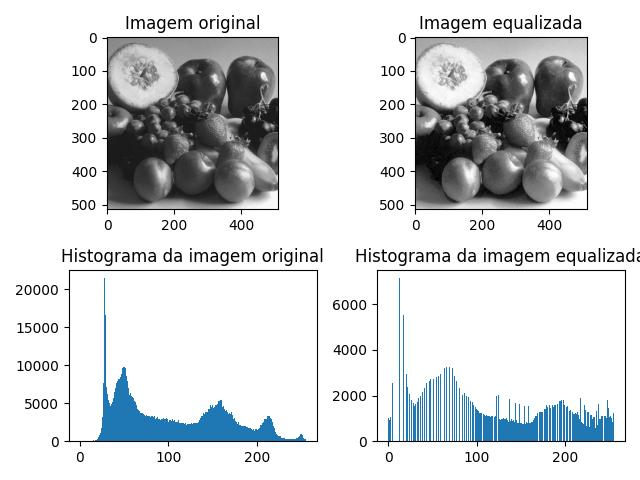
\includegraphics[scale=0.7]{images_generate/05/equalize_frutas.jpg}
    \caption{Figura gerada equalize\textunderscore frutas.jpg}
\end{figure}

\begin{figure}[H]
    \centering
    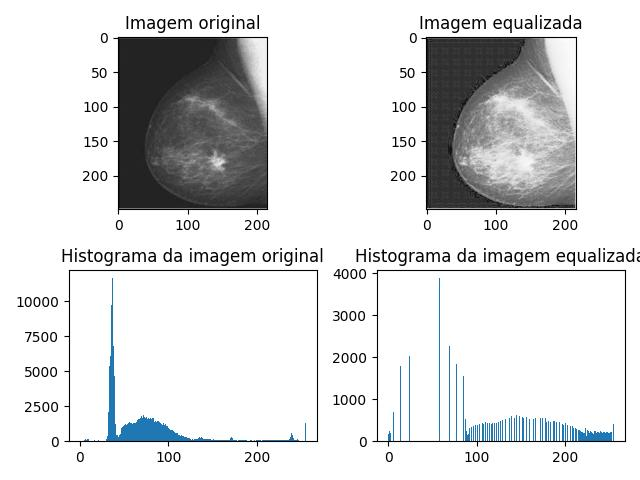
\includegraphics[scale=0.7]{images_generate/05/equalize_mammogram.jpg}
    \caption{Figura gerada equalize\textunderscore mammogram.jpg}
\end{figure}

\begin{figure}[H]
    \centering
    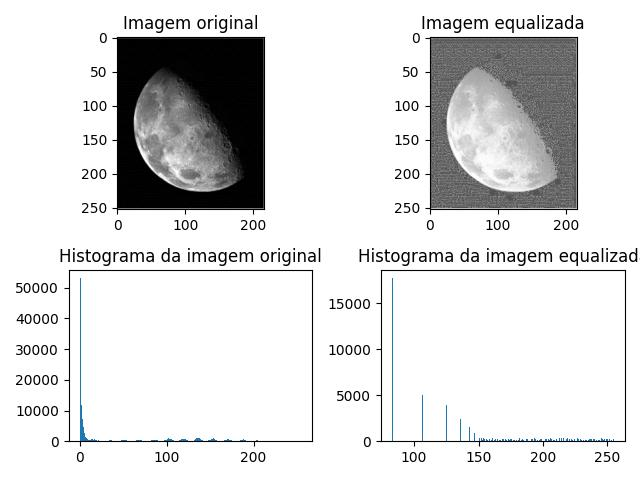
\includegraphics[scale=0.7]{images_generate/05/equalize_Moon.jpg}
    \caption{Figura gerada equalize\textunderscore Moon.jpg}
\end{figure}

\begin{figure}[H]
    \centering
    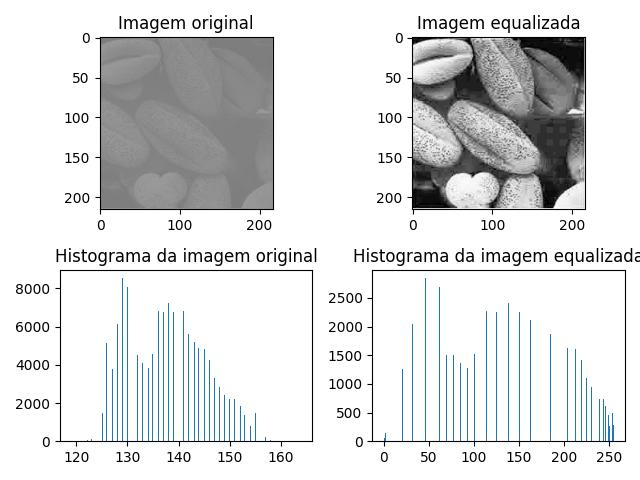
\includegraphics[scale=0.7]{images_generate/05/equalize_polem.jpg}
    \caption{Figura gerada equalize\textunderscore polem.jpg}
\end{figure}

\subsection{Explicação}

\begin{flushleft}
Para construir um programa em Python que realize a equalização de histograma em imagens, podemos utilizar a biblioteca OpenCV. Vamos seguir os seguintes passos:
\end{flushleft}

\begin{flushleft}    
1. Importar as bibliotecas necessárias, incluindo o OpenCV e o Matplotlib para plotar os histogramas.
\end{flushleft}

\begin{lstlisting}[language=Python]      
import cv2
import numpy as np
import matplotlib.pyplot as plt
\end{lstlisting}

\begin{flushleft}
2. Carregar a imagem desejada em escala de cinza, utilizando a função cv2.imread. (Criamos uma pasta chamada imagens e colocamos todas as imagens disponibilizadas lá dentro).
\end{flushleft}

\begin{lstlisting}[language=Python]       
# Carrega a imagem
img = cv2.imread('imagens/frutas.jpg', 0)
\end{lstlisting}

\begin{flushleft}
3. Calcular o histograma da imagem original, utilizando a função cv2.equalizeHist.
\end{flushleft}

\begin{lstlisting}[language=Python]    
# Realiza a equalização de histograma
equalized_img = cv2.equalizeHist(img)
\end{lstlisting}

\begin{flushleft}
4. Exibir a imagem original , bem como seus respectivo histograma.
\end{flushleft}

\begin{lstlisting}[language=Python]        
# Mostra as imagens original lado a lado
plt.subplot(2, 2, 1)
plt.imshow(img, cmap='gray')
plt.title('Imagem original')
plt.subplot(2, 2, 2)
plt.imshow(equalized_img, cmap='gray')
plt.title('Imagem equalizada')
\end{lstlisting}

\begin{flushleft}
5. Exibir a  imagem equalizada, bem como seus respectivo histograma.
\end{flushleft}

\begin{lstlisting}[language=Python]
# Mostra as imagens original e equalizada lado a lado
plt.subplot(2, 2, 3)
plt.hist(img.ravel(), 256, [0, 256])
plt.title('Histograma da imagem original')
plt.subplot(2, 2, 4)
plt.hist(equalized_img.ravel(), 256, [0, 256])
plt.title('Histograma da imagem equalizada')
\end{lstlisting}

\begin{flushleft}
6. Exibe as imagens.
\end{flushleft}

\begin{lstlisting}[language=Python]
plt.show()
\end{lstlisting}

\begin{flushleft}
O código em Python para realizar essas etapas pode ser o seguinte:
\end{flushleft}

\begin{lstlisting}[language=Python]
import cv2
import numpy as np
import matplotlib.pyplot as plt

# Carrega a imagem
img = cv2.imread('imagens/frutas.jpg', 0)

# Realiza a equalização de histograma
equalized_img = cv2.equalizeHist(img)

# Mostra as imagens original e equalizada lado a lado
plt.subplot(2, 2, 1)
plt.imshow(img, cmap='gray')
plt.title('Imagem original')
plt.subplot(2, 2, 2)
plt.imshow(equalized_img, cmap='gray')
plt.title('Imagem equalizada')

# Mostra os histogramas das imagens original e equalizada
plt.subplot(2, 2, 3)
plt.hist(img.ravel(), 256, [0, 256])
plt.title('Histograma da imagem original')
plt.subplot(2, 2, 4)
plt.hist(equalized_img.ravel(), 256, [0, 256])
plt.title('Histograma da imagem equalizada')

plt.show()
\end{lstlisting}

\begin{flushleft}
OBS: é refeito o processamento para cada imagem
\end{flushleft}

\pagebreak

\section{Realce - Exercício 9}

\subsection{Enunciado}

Considere a imagem (e) com ruído gaussiano, exercício 3 da Aula 4, e aplique a \textit{correção gama} com c=1 e \( {\gamma} (0.04; 0.4; 2,5; 10)\). Visualmente, esse tipo de realce permitiu melhorar a qualidade da imagem com ruído? Caso sim, indique o valor de \({\gamma}\) e o apromixado da correção. Em seguida, calcule ao menos duas métricas indicadas no exercício 4 (Aula 4) e avalie se é possível comprovar quantitativamente as verificações iniciais. Por fim, conclua sobre a efetividade do realce para corrigir a imagem degradada.

\subsection{Código Fonte}

\lstinputlisting[language=Python]{sources/06_highlight_gamma.py}

\subsection{Saída}

\lstinputlisting[language=Bash]{outputs/06_highlight_gamma.txt}

\begin{figure}[H]
    \centering
    \subfloat[\centering imagem\textunderscore corrigida\textunderscore y=0.04.jpg]{
    {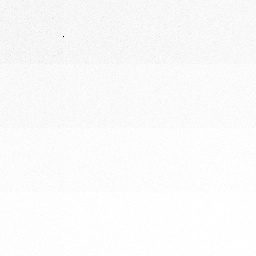
\includegraphics[width=3cm]{images_generate/06/imagem_corrigida_y=0.04.jpg}}}%
    \qquad
    \subfloat[\centering imagem\textunderscore corrigida\textunderscore y=0.4.jpg]{
    {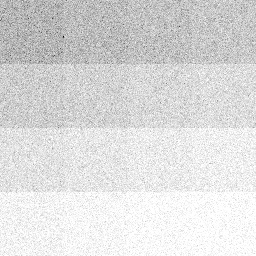
\includegraphics[width=3cm]{images_generate/06/imagem_corrigida_y=0.4.jpg}}}%
    \qquad
    \subfloat[\centering imagem\textunderscore corrigida\textunderscore y=2.5.jpg]{
    {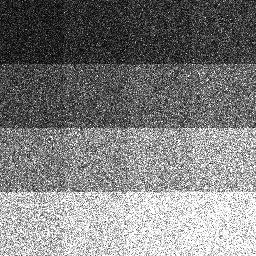
\includegraphics[width=3cm]{images_generate/06/imagem_corrigida_y=2.5.jpg}}}%
    \qquad
    \subfloat[\centering imagem\textunderscore corrigida\textunderscore y=10.jpg]{
    {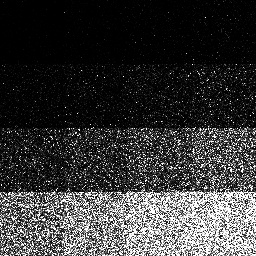
\includegraphics[width=3cm]{images_generate/06/imagem_corrigida_y=10.jpg}}}%
\end{figure}

\subsection{Explicação}

\begin{flushleft}
1. Novamente foi necessário a biblioteca OpenCV:
\end{flushleft}

\begin{lstlisting}[language=Python]
import cv2
import numpy as np
import os
\end{lstlisting}

\begin{flushleft}
2.	Carregamos a imagem (e) com ruído gaussiano, exercício 3 da Aula 4
\end{flushleft}

\begin{lstlisting}[language=Python]
img = cv2.imread("./images/e_noise_gaussian.bmp")
\end{lstlisting}

\begin{flushleft}
3.	Aplicamos a correção Gama com diferentes valores de y
\end{flushleft}

\begin{lstlisting}[language=Python]
y_values = [0.04, 0.4, 2.5, 10]
for y in y_values:
    corrected_img = np.power(img / 255., y)
    corrected_img = np.uint8(corrected_img * 255)
\end{lstlisting}

\begin{flushleft}
4.	As imagens geradas com os resultados da correção Gama foram gravas pasta images
\end{flushleft}

\begin{lstlisting}[language=Python]
# Salva a imagem corrigida
cv2.imwrite(f"./images/imagem_corrigida_y={y}.jpg", corrected_img)   
\end{lstlisting}

\begin{flushleft}
As imagens geradas são exibidas na subseção Saída.Sendo que destas, a imagem com o nome de imagem\textunderscore corrigida\textunderscore y=0.4 obteve o melhor resultado,  utilizando-se  o valor y=0.4 como valor aproximado de correção.
\end{flushleft}

\begin{flushleft}
5. Optamos por utilizar as métricas erro médio absoluto (MAE) e o erro médio quadrático (MSE) para comprovar quantitativamente as verificações iniciais. Para tanto utilizamos o código abaixo:
\end{flushleft}

\begin{lstlisting}[language=Python]
# Aplicando duas métricas do exercicio 4 aula 4
# Carrega a imagem original degradada com ruído gaussiano
original_img = cv2.imread("./images/e_noise_gaussian.bmp")

# Carrega a imagem com tratamento gama
noisy_img = cv2.imread("./images/imagem_corrigida_y=0.4.jpg")

# Aplica a correção gama com um valor de y
y = 0.4
corrected_img = np.power(noisy_img / 255., y)
corrected_img = np.uint8(corrected_img * 255)

# Calcula o erro médio absoluto (MAE)
mae = np.mean(np.abs(corrected_img - original_img))

# Calcula o erro médio quadrático (MSE)
mse = np.mean((corrected_img - original_img)**2)

print_out(f"MAE: {mae}")
print_out(f"MSE: {mse}")
\end{lstlisting}

\begin{flushleft}
6.	Por fim, concluímos ser a efetiva a aplicação do realce para corrigir a imagem degradada tendo em vista que a saída do erro médio absoluto (MAE) e do erro médio quadrático (MSE)  se apresentaram menores do que os valores correspondentes na imagem degradada. Conforme valores apresentado na subseção Saída.
\end{flushleft}

\pagebreak

\section{Filtragem - Exercício 4}

\subsection{Enunciado}

\begin{flushleft}
Crie um programa para gerar discretamente máscaras 3x3, 5x5 e 7x7, representativas de filtros gaussianos. Use os coeficientes da expansão binomial de Newton. Para cada máscara, calcule o valor de \({\sigma}\).
\end{flushleft}

\subsection {Código Fonte}

\lstinputlisting[language=Python]{sources/07_filtering.py}

\subsection{Saída}

\lstinputlisting[language=Bash]{outputs/07_filtering.txt}

\subsection{Explicação}

\begin{flushleft}
Nesse exercício buscou-se aplicar a geração Gaussiana discreta com média em 0,0 e desvio padrão {(\(\sigma\)=1)}, representando os filtro com coeficientes de expansão binomial de Newton, para isso fizemos 4 passos: 
\end{flushleft}

\begin{enumerate}[label=\alph*.]
   \item Foi criada uma função de gerador de filtro gaussiano que recebesse como parâmetros o tamanho e o valor de sigma;
   \item a função primeiramente foi calculado os coeficientes da expansão binomial de Newton;
   \item Posteriormente foi calculado a máscara gaussiana, depois foi aplicado a expansão binomial para aproximar a máscara gaussiana;
   \item Daí sim calculado a variância (largura) da máscara gaussiana para isso foi utilizado o representativo da expressão matemática: largura =\(\sum{((i - c)^2 *}\) \(\sum{(m_i,j))}\) , onde i,j são índices de linha e coluna da máscara, c é o índice central, m é a matriz da máscara e \(\sum\) representa a soma;
   \item Por fim foi chamar a função utilizando-se os parâmetros de máscara 3x3, 5xx5, 7x7. Com sigma utilizando-se de padrão 1.
\end{enumerate}

\begin{flushleft}
Esses experimentos devem ser realizados com os ruídos gaussiano e poisson (shot noise) ou salt-and-pepper noise. 
\end{flushleft}

\pagebreak

\section{Filtragem Espacial - Exercício 6}

\subsection{Enunciado}

\begin{flushleft}
Aplique sobre a imagem (e) os ruídos aditivos: sal e pimenta e gaussiano. As distribuições devem ser fornecidas pelo usuário. Aplique os filtros apresentados abaixo.
\end{flushleft}

\begin{figure}[H]
    \centering
    \subfloat[\centering a]{{
\includegraphics[width=2cm]{images_original/a.jpg}}}%
    \qquad
    \subfloat[\centering b]{{
\includegraphics[width=2cm]{images_original/b.jpg}}}%
    \qquad
    \subfloat[\centering ]{{
\includegraphics[width=2cm]{images_original/c.jpg}}}%
    \qquad
    \subfloat[\centering d]{{
\includegraphics[width=2cm]{images_original/d.jpg}}}%
    \qquad
    \subfloat[\centering e]{{
\includegraphics[width=2cm]{images_original/e.jpg}}}%
\end{figure}

\begin{flushleft}
a) Suavização da imagem (\textit {Média, Mediana, Gaussiano e Moda}) com janelas (w) 3x3;
\end{flushleft}

\begin{flushleft}
b) Filtro Passa-Alta com as máscaras:
\end{flushleft}

\begin{figure}[H]
    \centering
    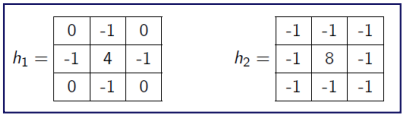
\includegraphics{images_original/08/Filtragem - matriz.png}
\end{figure}

\begin{flushleft}
c) Considerando \textit{i} como sendo cada imagem dada como entrada, determine qual filtro indicou o melhor resultado visual 
\textit{î}. Em seguida, use uma métrica para avaliar a qualidade de \textit{î} e confirmar sua hipótese
\end{flushleft}

\subsection{Código Fonte}

\begin{flushleft}
Segue o código para aplicar o ruído sal e pimenta e gaussiano na imagem e.bmp
\end{flushleft}

\lstinputlisting[language=Python]{sources/08_noise.py}

\begin{flushleft}
a) Suavização da imagem (\textit {Média, Mediana, Gaussiano e Moda}) com janelas (w) 3x3;
\end{flushleft}

\lstinputlisting[language=Python]{sources/08_a.py}

\begin{flushleft}
b) Filtro Passa-Alta com as máscaras:
\end{flushleft}

\begin{figure}[H]
    \centering
    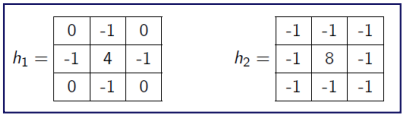
\includegraphics{images_original/08/Filtragem - matriz.png}
\end{figure}

\lstinputlisting[language=Python]{sources/08_b.py}

\begin{flushleft}
c) Considerando \textit{i} como sendo cada imagem dada como entrada, determine qual filtro indicou o melhor resultado visual \textit{î}. Em seguida, use uma métrica para avaliar a qualidade de \textit{î} e confirmar sua hipótese
\end{flushleft}

\lstinputlisting[language=Python]{sources/08_c.py}

\subsection{Explicação}

\begin{flushleft}
O código contém duas funções:
\end{flushleft}

\begin{itemize}
    \item {\ttfamily ruido\textunderscore sal\textunderscore pimenta (nome):} - recebe como parâmetro o nome do arquivo que será aplicado o ruído sal e pimenta e a imagem gerada é salva em disco.
    \item {\ttfamily ruido\textunderscore gaussiano(nome):}  - recebe como parâmetro o nome do arquivo que será aplicado o ruído gaussiano e a imagem gerada é salva em disco.
\end{itemize}

\begin{flushleft}
As duas funções são executadas utlizando como parâmetro a imagem e.bmp. Após a execução do codigo para aplicar o ruído sal e pimenta e gaussiano na imagem e. bmp duas imagens são geradas \textbf{e\textunderscore ruido\textunderscore salpimenta.bmp} e  \textbf{e\textunderscore ruido\textunderscore gaussiano.bmp} 
\end{flushleft}

\begin{figure}[H]
    \centering
    \subfloat[\centering Ruído sal e pimenta]{{\includegraphics[width=6cm] {images_generate/03/e_ruido_salpimenta.jpg}}}%
    \qquad
    \subfloat[\centering Ruído gaussiano]{{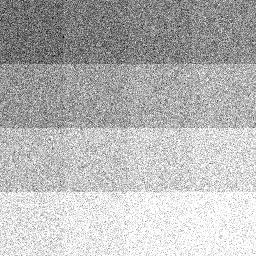
\includegraphics[width=6cm]{images_generate/03/e_noise_gaussian.jpg}}}%
\end{figure}

\begin{flushleft}
a) Suavização da imagem (\textit {Média, Mediana, Gaussiano e Moda}) com janelas (w) 3x3;
\end{flushleft}

\begin{flushleft}
O código contém quatro funções:
\end{flushleft}

\begin{itemize}
    \item {\ttfamily suavizacao\textunderscore media(nome):}
    \item {\ttfamily suavizacao\textunderscore mediana(nome):}
    \item {\ttfamily suavizacao\textunderscore gausiano(nome):}
    \item {\ttfamily suavizacao\textunderscore moda (nome):}
\end{itemize}

\begin{flushleft}
As funções acima requer como parâmentro o nome que é a imagem que será aplicada as suavizações específicas. Cada função é executada duas vezes, uma vez com a imagem \textbf{e\textunderscore ruido\textunderscore salpimenta.bmp} e outra para a imagem \textbf{e\textunderscore ruido\textunderscore gaussiano.bmp}
\end{flushleft}

\begin{flushleft}
Para a imagem \textbf{e\textunderscore ruido \textunderscore salpimenta.bmp} as seguinte imagens são geradas.
\end{flushleft}

\begin{figure}[H]
    \centering
    \subfloat[\centering Média]{{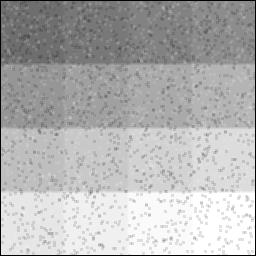
\includegraphics[width=3cm]{images_generate/08/e_ruido_salpimenta_Suavizacao_media.jpg}}}%
    \qquad
    \subfloat[\centering Mediana]{{
\includegraphics[width=3cm]{images_generate/08/e_ruido_salpimenta_Suavizacao_mediana.jpg}}}%
    \qquad
    \subfloat[\centering Gaussiano]{{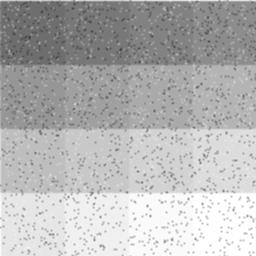
\includegraphics[width=3cm]{images_generate/08/e_ruido_salpimenta_Suavizacao_gaussiano.jpg}}}%
    \qquad
    \subfloat[\centering Moda]{{
\includegraphics[width=3cm]{images_generate/08/e_ruido_salpimenta_Suavizacao_moda.jpg}}}%
\end{figure}

\begin{flushleft}
Para a imagem \textbf{e\textunderscore ruido \textunderscore gausiano.bmp} as seguinte imagens são geradas.
\end{flushleft}

\begin{figure}[H]
    \centering
    \subfloat[\centering Média]{{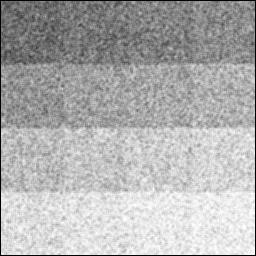
\includegraphics[width=3cm]{images_generate/08/e_ruido_gaussiano_Suavizacao_media.jpg}}}%
    \qquad
    \subfloat[\centering Mediana]{{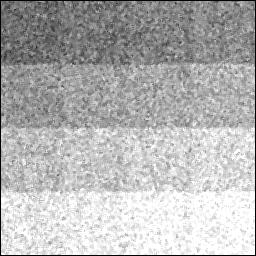
\includegraphics[width=3cm]{images_generate/08/e_ruido_gaussiano_Suavizacao_mediana.jpg}}}%
    \qquad
    \subfloat[\centering Gaussiano]{{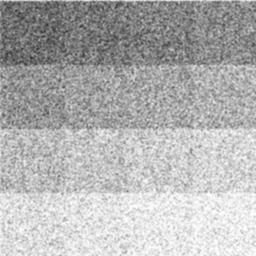
\includegraphics[width=3cm]{images_generate/08/e_ruido_gaussiano_Suavizacao_gaussiano.jpg}}}%
    \qquad
    \subfloat[\centering Moda]{{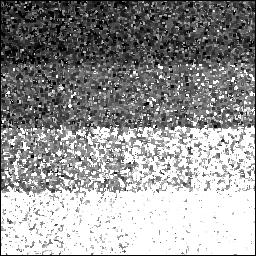
\includegraphics[width=3cm]{images_generate/08/e_ruido_gaussiano_Suavizacao_moda.jpg}}}%
\end{figure}

\begin{flushleft}
b) Filtro Passa-Alta com as máscaras:
\end{flushleft}

\begin{figure}[H]
    \centering
    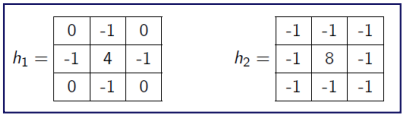
\includegraphics{images_original/08/Filtragem - matriz.png}
\end{figure}

\begin{flushleft}
O código contém a função {\ttfamily filtro\textunderscore passa\textunderscore alta\textunderscore com\textunderscore mascara(nome):} que tem como parâmetro de entrada o nome do arquvio e gera duas imagens para cada filtro definida h\textsubscript{1} e h\textsubscript{2}.
\end{flushleft}

\begin{flushleft}
A função é executada duas vezes tendo como imagens de entrada  \textbf{e\textunderscore ruido\textunderscore salpimenta.bmp} e outra para a imagem \textbf{e\textunderscore ruido\textunderscore gaussiano.bmp}. Assim gerando as seguintes imagens.
\end{flushleft}

\begin{flushleft}
Para a imagem \textbf{e\textunderscore ruido\textunderscore salpimenta.bmp} as seguinte imagens são geradas.
\end{flushleft}

\begin{figure}[H]
    \centering
    \subfloat[\centering e\textunderscore ruido\textunderscore salpimenta.bmp - Máscara h\textsubscript{1}]{{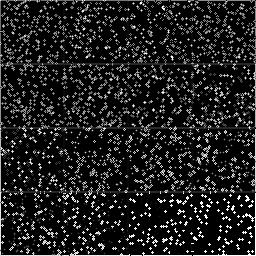
\includegraphics[width=6cm]{images_generate/08/e_ruido_salpimenta_Suavizacao_passa_alta_h1}}}%
    \qquad
    \subfloat[\centering e\textunderscore ruido\textunderscore salpimenta.bmp - Máscara h\textsubscript{2}]{{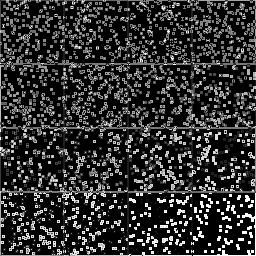
\includegraphics[width=6cm]{images_generate/08/e_ruido_salpimenta_Suavizacao_passa_alta_h2}}}%
\end{figure}

\begin{flushleft}
Para a imagem \textbf{e\textunderscore ruido \textunderscore gaussiano.bmp} as seguinte imagens são geradas.
\end{flushleft}

\begin{figure}[H]
    \centering
    \subfloat[\centering e\textunderscore ruido\textunderscore gaussiano.bmp - Máscara h\textsubscript{1}]{{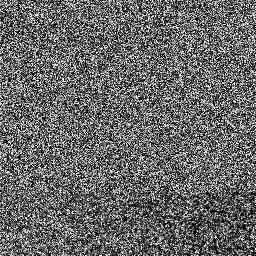
\includegraphics[width=6cm]{images_generate/08/e_ruido_gaussiano_Suavizacao_passa_alta_h1}}}%
    \qquad
    \subfloat[\centering e\textunderscore ruido\textunderscore gaussiano.bmp - Máscara h\textsubscript{2}]{{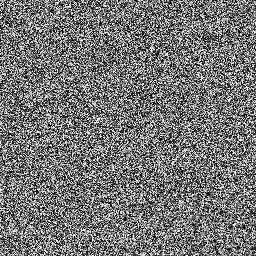
\includegraphics[width=6cm]{images_generate/08/e_ruido_gaussiano_Suavizacao_passa_alta_h2}}}%
\end{figure}

\begin{flushleft}
c) Considerando\textsubscript{ }\textit{i} como sendo cada imagem dada como entrada, determine qual filtro indicou o melhor resulta\textsubscript{d}o visual \textit{î}. Em seguida, use uma métrica para avaliar a qualidade de \textit{î} e confirmar sua hipótese
\end{flushleft}

\begin{itemize}
    \item {\ttfamily resultado visual} - O filtro de suavização mediana se demonstrou como melhor resultado visual.
    \item {\ttfamily métrica:}  : A métrica MAE (Mean Absolute Error) é usada para avaliar a diferença média absoluta entre duas imagens. Em nosso experimento aplicamos o filtro de mediana em uma imagem, e a diferença entre a imagem original e a imagem filtrada  foi menor em comparação com outros filtros. Isso ocorre porque o filtro de mediana é capaz de remover o ruído da imagem de forma mais eficaz, preservando a nitidez e os detalhes importantes. O resultado resultaod de nosso código foi: \textbf{2.9611663818359375} valor considerado baixo em comparação com a imagem original.
    \item {\ttfamily Conclusão:}  O filtro de mediana é um filtro não linear que é comumente usado para remover ruídos de uma imagem. Quando uma imagem é corrompida com ruído, o filtro de mediana é capaz de preservar melhor os detalhes importantes da imagem, em comparação com outros filtros (Média, Gaussiano e Moda).
\end{itemize}

\pagebreak

\section{Modelo de Cores - Exercício 3}

\subsection{Enunciado}

\begin{flushleft}
Escreva um programa que receba as imagens abaixo, converta para o padrão HSI e aplique a equalização de histograma. Apresentar os histogramas equalizados.
\end{flushleft}

\begin{figure}[H]
    \centering
    \subfloat[\centering Img1.bmp]{{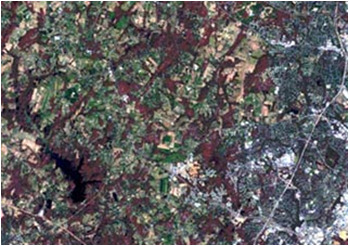
\includegraphics[width=5cm]{images_original/09/Img1.jpg}}}%
    \qquad
    \subfloat[\centering Img2.bmp]{{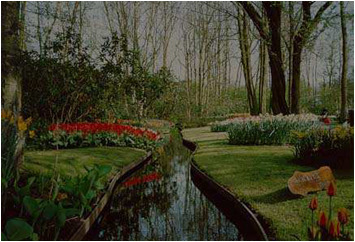
\includegraphics[width=5cm]{images_original/09/Img2.jpg}}}%
    \qquad
    \subfloat[\centering Img3.bmp]{{\includegraphics[width=4cm]{images_original/09/Img3.jpg}}}%
    \qquad
\end{figure}

\subsection{Código Fonte}

\lstinputlisting[language=Python]{sources/09_colors.py}

\subsection{Saída}

Segue as imagens geradas a partir da Img1.bmp

\begin{figure}[H]
    \centering
    \subfloat[\centering HSI]{{\includegraphics[width=4cm]{images_generate/09/Img1_HSI.jpg}}}%
    \qquad
    \subfloat[\centering Equalizada]{{\includegraphics[width=4cm]{images_generate/09/Img1_equalizada.jpg}}}%
    \qquad
    \subfloat[\centering Histograma]{{\includegraphics[width=4cm]{images_generate/09/Img1_histograma_equalizado.jpg}}}%
    \qquad
\end{figure}

Segue as imagens geradas a partir da Img2.bmp

\begin{figure}[H]
    \centering
    \subfloat[\centering HSI]{{\includegraphics[width=4cm]{images_generate/09/Img2_HSI.jpg}}}%
    \qquad
    \subfloat[\centering Equalizada]{{\includegraphics[width=4cm]{images_generate/09/Img2_equalizada.jpg}}}%
    \qquad
    \subfloat[\centering Histograma]{{\includegraphics[width=4cm]{images_generate/09/Img2_histograma_equalizado.jpg}}}%
    \qquad
\end{figure}

Segue as imagens geradas a partir da Img3.bmp

\begin{figure}[H]
    \centering
    \subfloat[\centering HSI]{{\includegraphics[width=4cm]{images_generate/09/Img3_HSI.jpg}}}%
    \qquad
    \subfloat[\centering Equalizada]{{\includegraphics[width=4cm]{images_generate/09/Img3_equalizada.jpg}}}%
    \qquad
    \subfloat[\centering Histograma]{{\includegraphics[width=4cm]{images_generate/09/Img3_histograma_equalizado.jpg}}}%
    \qquad
\end{figure}

\subsection{Explicação}

O código contém cinco funções:

\begin{itemize}
    \item {\ttfamily bmp\textunderscore to\textunderscore hsi(input\textunderscore file, output\textunderscore file):} é necessária para converter a imagem original em HSI, executada na função {\ttfamily rgb\textunderscore to\textunderscore hsi(rgb):}
    \item {\ttfamily rgb\textunderscore to\textunderscore hsi(rgb):} converte uma imagem no padrão BMP para o padrão HSI
    \item {\ttfamily equalize\textunderscore image(nome):} equaliza a imgem 
    \item {\ttfamily gera\textunderscore histograma(nome):} gera o histograma da imagem equalizada
    \item {\ttfamily executa\textunderscore exercicio (nome):} essa função executa três funções ( {\ttfamily rgb\textunderscore to\textunderscore hsi(rgb):}, {\ttfamily equalize\textunderscore image(nome):} , {\ttfamily gera\textunderscore histograma(nome):} ) ela é executada 3 vezes uma para cada imagem gerando a cada execução 3 imagens mostrada na sub-seção Saída
\end{itemize}

\pagebreak

\section{Filtragem e Domínio da Frequência - Exercício 2}

\subsection{Enunciado}

Para facilitar a elaboração dessa atividade, converta a imagem abaixo para níveis de cinza, 8 bits de quantização. Aplique o ruído gaussiano sobre a imagem. Em seguida, aplique a DFT sobre a imagem com ruído. Apresente o espectro de Fourier com o deslocamento da origem do plano de frequências. Proponha dois filtros no domínio da frequência. O objetivo é suavizar o ruído inserido previamente. Apresente os espectros de Fourier antes e após a etapa de processamento, bem como as imagens reconstruídas após cada processo de filtragem. Explique detalhadamente cada etapa e os filtros propostos. Indique qual foi o filtro que forneceu o melhor resultado em termos de minimização da presença. É permitido o uso de pacote DFT, disponível em ferramentas de PDI, a fim de facilitar o processamento da transformada e exibição de cada espectro. Não é permitido o uso de filtros disponíveis em ferramentas de PDI.

\begin{figure}[H]
    \centering
    \includegraphics[scale=0.9]{images_original/10/img_exercicio2.png}
    \caption{img\textunderscore exercicio2.png}
\end{figure}

\subsection{Código Fonte}

\lstinputlisting[language=Python]{sources/10_frequency.py}

\subsection{Explicação}

O código fonte possui 5 funções:

\begin{itemize}
    \item {\ttfamily conversao\textunderscore cinza():} recebe uma imagem como entrada e converte para cinza
    \item {\ttfamily ruido\textunderscore gaussiano():} aplica o ruído gaussiano e salva a imagem com ruído
    \item {\ttfamily img\textunderscore DFT():} aplica o DFT sobre a imagem com ruído
    \item {\ttfamily deslocamento\textunderscore frequencias( ):}
    \item {\ttfamily filtros\textunderscore dominio\textunderscore frequencia\textunderscore 2( ):} 
\end{itemize}

Para facilitar a elaboração dessa atividade, converta a imagem abaixo para níveis de cinza, 8 bits de quantização, assim após a execução da função {\ttfamily conversao\textunderscore cinza():}  a imagem abaixo é gerada.

\begin{figure}[H]
    \centering
    \includegraphics[scale=0.5]{images_generate/10/img_exercicio2_cinza_8bits.png}
    \caption{img\textunderscore exercicio2\textunderscore cinza\textunderscore 8bits.png}
\end{figure}

Aplicanos o ruído gaussiano sobre a imagem em tons de cinza através da função {\ttfamily ruido\textunderscore gaussiano():}, assim a imagem abaixo é gerada.

\begin{figure}[H]
    \centering
    \includegraphics[scale=0.5]{images_generate/10/img_exercicio2_gaussiano.png}
    \caption{img\textunderscore exercicio2\textunderscore gaussiano.png}
\end{figure}

Em seguida, a DFT sobre a imagem com ruído, através da função{\ttfamily img\textunderscore DFT():}

\begin{figure}[H]
    \centering
    \includegraphics[scale=0.5]{images_generate/10/img_exercicio2_dft.png}
    \caption{img\textunderscore exercicio2\textunderscore dft.png}
\end{figure}

Apresentamos o espectro de Fourier com o deslocamento da origem do plano de frequências, através da execução da função {\ttfamily deslocamento\textunderscore frequencias( ):}

\begin{figure}[H]
    \centering
    \includegraphics[scale=0.5]{images_generate/10/img_exercicio2_desloamento_frequencia.png}
    \caption{img\textunderscore exercicio2\textunderscore deslocamento\textunderscore frequencia.png}
\end{figure}

Aplicamos o filtro média e gaussiano no domínio da frequência através da função {\ttfamily filtros\textunderscore dominio\textunderscore frequencia\textunderscore 2( ):} gerando a imagem abaixo

\begin{figure}[H]
    \centering
    \includegraphics[scale=0.5]{images_generate/10/img_exercicio2_final.png}
    \caption{img\textunderscore exercicio2\textunderscore final.png}
\end{figure}

\begin{enumerate}
    \item Carregamos a imagem com ruído: A primeira etapa é carregar a imagem original em tons de cinza com ruído gaussiano. Essa imagem é usada como entrada para o processo de filtragem.
    \item Cálculo do espectro de Fourier: A segunda etapa é calcular o espectro de Fourier da imagem original. O espectro de Fourier é uma representação da imagem no domínio da frequência. Ele pode ser usado para identificar a presença de ruído em diferentes frequências.
    \item Aplicação do filtro de média: Um dos filtros mais comuns para remover ruído gaussiano é o filtro de média. Esse filtro funciona calculando a média dos valores de pixel em uma vizinhança em torno de cada pixel da imagem. O resultado é uma imagem suavizada, com o ruído reduzido. Neste exemplo, usamos um filtro de média com uma janela de 3x3 pixels.
    \item Cálculo do espectro de Fourier da imagem suavizada: O espectro de Fourier da imagem suavizada é calculado para comparar com o espectro da imagem original e observar a redução do ruído nas diferentes frequências.
    \item Aplicação do filtro gaussiano: Outro filtro comum para remover ruído gaussiano é o filtro gaussiano. Esse filtro é baseado na convolução da imagem com uma função gaussiana. A função gaussiana é uma função de distribuição de probabilidade que modela a distribuição de ruído gaussiano. O filtro gaussiano tem a propriedade de preservar melhor as bordas e detalhes da imagem em comparação com o filtro de média. Neste exemplo, usamos um filtro gaussiano com um desvio padrão de 1.5 pixels.
    \item Cálculo do espectro de Fourier da imagem com filtro gaussiano: O espectro de Fourier da imagem filtrada com o filtro gaussiano é calculado para comparar com os espectros da imagem original e suavizada.
    \item Reconstrução da imagem filtrada: Após a aplicação dos filtros, as imagens filtradas podem ser reconstruídas a partir dos espectros de Fourier. Isso é feito aplicando a transformada inversa de Fourier (IFFT) aos espectros filtrados. As imagens resultantes são as imagens filtradas. 
    \item Visualização dos resultados: Para visualizar os resultados, podemos mostrar as imagens originais e filtradas, juntamente com os espectros de Fourier correspondentes. Isso permite avaliar a qualidade da filtragem e comparar os diferentes filtros usados.
\end{enumerate}

O melhor filtro foi o Média, pois trouxe maior semelhança com a imagem original.

\pagebreak

\section{Segmentação - Exercício 2}

\subsection{Enunciado}
Dada a imagem à baixo, desenvolva um método capaz de segmentar as regiões “circulares” em azul/violeta. Descreva cada etapa utilizada para caracterizar o método. Em seguida, considere algumas regiões de controle e calcule as taxas de acerto e erro do método. O programa deve fornecer como saída uma imagem com as regiões circulares segmentadas e as taxas obtidas.

\begin{figure}[H]
    \centering
    \includegraphics[scale=0.8]{images_original/11/Img_seg.jpg}
    \caption{Img\textunderscore seg.jpg}
\end{figure}

\subsection{Código Fonte}

\lstinputlisting[language=Python]{sources/11_segmentation.py}

\subsection{Saída}

A imagem é gerada.

\begin{figure}[H]
    \centering
    \includegraphics{images_generate/11/Img_seg_segmentada.jpg}
    \caption{Img\textunderscore seg\textunderscore segmentada.jpg}
\end{figure}

\lstinputlisting[language=Bash]{outputs/11_segmentation.txt}

\subsection{Explicação}

Passos: 

\begin{enumerate}
    \item Pré-processamento da imagem
    \item Detecção de borda
    \item Segmentação baseada em região
    \item Pós-processamento:
\end{enumerate} 

Assim sendo o código irá realizar a segmentação de uma imagem utilizando operações de processamento de imagens. Ele carrega uma imagem de entrada em formato JPG, converte-a para um array numpy e separa os canais de cor vermelho e azul. Em seguida, é calculada a diferença entre os valores dos canais azul e vermelho para destacar a região de interesse. 

A imagem é então limiarizada e passa por uma operação de abertura para remover ruídos. A operação de abertura é realizada utilizando um kernel definido como uma matriz de 5x5 elementos com valores iguais a 1. 

Após a operação de abertura, são encontrados os contornos na imagem limiarizada utilizando o algoritmo de detecção de contornos em imagens binárias. Os contornos encontrados são armazenados em uma lista. 

Foi considerada algumas regiões de controle e calculou as taxas de acerto e erro do método. 

Para entender melhor:

A acurácia mede a proporção de classificações corretas em relação ao número total de exemplos de teste. No caso em questão, uma acurácia de 1.00 significa que todas as classificações feitas pelo modelo estavam corretas.
 
Já a precisão mede a proporção de exemplos positivos classificados corretamente em relação ao número total de exemplos classificados como positivos. Uma precisão de 0.00 significa que nenhum exemplo classificado como positivo estava realmente correto.
 
Por fim, o recall (ou taxa de verdadeiros positivos) mede a proporção de exemplos positivos classificados corretamente em relação ao número total de exemplos positivos na base de teste. Um recall de 0.00 significa que o modelo não conseguiu identificar nenhum exemplo positivo corretamente. 

Por fim, o código desenha os contornos encontrados na imagem original e salva a imagem segmentada em um arquivo com o nome "Img\textunderscore seg\textunderscore segmentada.jpg". 

\pagebreak

\section{Morfologia Matemática - Exercício 4}

\subsection{Enunciado}

\begin{flushleft}
Construa um programa que receba a imagem A, forneça uma imagem limiarizada parecida com a indicada em B. Caso necessário, considere o método de Otsu para obter a solução mais apropriada. Em seguida, aplique a operação morfológica necessária para obter um resultado similar ao indicado em C.
\end{flushleft}

\begin{figure}[H]
    \centering
    \subfloat[\centering Entrada ]{{\includegraphics[width=4cm]{images_generate/12/Img4.jpg}}}%
    \qquad
    \subfloat[\centering Limiarização]{{\includegraphics[width=4cm]{images_generate/12/MM - b.jpg}}}%
    \qquad
    \subfloat[\centering Morfológica]{{\includegraphics[width=4cm]{images_generate/12/MM - c.jpg}}}%
    \qquad
\end{figure}

\subsection{Código Fonte}

\lstinputlisting[language=Python]{sources/12_morphology.py}

\subsection{Explicação}

\begin{flushleft}
Geramos a imagem limiarizada usando T igual 220 na função {\ttfamily limiarizacao (entrada, saida):} que recebe como entrada a imagem de entrada img4.bmp e após salva a imagem limiarizada de saída como o nome imgB.bmp quando é executada {\ttfamily limiarizacao ("img4.bmp", "imgB.bmp"):} 
\end{flushleft}

\begin{flushleft}
Assim a imagem gerada é a imgB.bmp.
\end{flushleft}

\begin{figure}[H]
    \centering
    \includegraphics{images_generate/12/imgB.jpg}
    \caption{imgB.bmp}
\end{figure}

\begin{flushleft}
A partir da imagem limiarizada aplicamos o elemento estruturante MORPH\textunderscore ELLIPSE com tamnaho (3,3) e aplicamos 4 iterações aplicando como morfologia matemática a transformação morfológica de erosão através da funcao {\ttfamily operacao\textunderscore morfologica (entrada, saida): } que recebe a imagem limiarizada como entrada com o nome imgb.bmp e a imagem de saída é gerada e salva como o nome eroded\textunderscore imgB.bmp quando é executada {\ttfamily operacao\undercose morfologica("imgB.bmp","eroded\textunderscore imgB.bmp")}
\end{flushleft}

\begin{flushleft}
Assim a imagem gerada é a eroded\textunderscore imgB.bmp.
\end{flushleft}

\begin{figure}[H]
    \centering
    \includegraphics{images_generate/12/eroded_imgB.jpg}
    \caption{eroded\textundercose imgB.jpg}
\end{figure}

\pagebreak

\section{Análise de Textura}

\subsection{Enunciado}

\begin{flushleft}
Construa um código para receber imagens monocromáticas como entrada, 8 bits de quantização. O código deve ser capaz de fornecer os valores de:
\end{flushleft}

\begin{flushleft}
- Haralick, com segundo momento angular, entropia e contraste. Use d=1 e \theta=0;
\end{flushleft}

\begin{flushleft}
- LBP (especificar as condições utilizadas);
\end{flushleft}

\begin{flushleft}
- Dimensão fractal (DF), usando Box-couting. A DF deve ser definida via coeficiente angular da regressão log x log. Os dois primeiros valores parciais de DF, em função das iterações 1 e 2, também devem ser apresentados.
\end{flushleft}

\begin{flushleft}
Os descritores devem ser organizados como vetores de características, respeitando a ordem posicional: momento angular; entropia; contraste; LBP; DF (coeficiente logxlog); DF iteração 1; DF iteração 2.
\end{flushleft}

\begin{flushleft}
Apresente os vetores para cada imagem. As imagens são apresentadas nos próximos slides.
\end{flushleft}

\begin{flushleft}
Em seguida, observe os resultados numéricos e indique quais descritores apresentam as maiores diferenças para separar as imagens R0 de R3. Apresente os gráficos para ilustrar as posições espaciais dos descritores. Por exemplo, eixo x representa momento angular, eixo y a entropia e eixo z o contraste. Use a mesma estratégia para DF. Cada imagem é um ponto espacial em função das suas coordenadas/descritores. Quais as dificuldades neste tipo de análise? Quais as soluções?
\end{flushleft}

\subsection{Código Fonte}

\subsubsection{Haralick, com segundo momento angular, entropia e contraste. Use d=1 e \theta=0}

\lstinputlisting[language=Python]{sources/13_texture_a.py}

\subsubsection{LBP (especificar as condições utilizadas)}

\lstinputlisting[language=Python]{sources/13_texture_b.py}

\subsubsection{Dimensão fractal (DF), usando Box-couting. A DF deve ser definida via coeficiente angular da regressão log x log. Os dois primeiros valores parciais de DF, em função das iterações 1 e 2, também devem ser apresentados}

\lstinputlisting[language=Python]{sources/13_texture_c.py}

\subsection{Explicação}

\subsubsection{Haralick, com segundo momento angular, entropia e contraste. Use d=1 e  \theta =0}

\begin{flushleft}
Apresentando os seguintes resultados:
\end{flushleft}

\lstinputlisting[language=Bash]{outputs/13_texture_a.txt}

\subsubsection{LBP (especificar as condições utilizadas)}

\begin{flushleft}
Apresentando a imagem abaixo: com Raio = 1 e número de pontos = 8 
\end{flushleft}

\begin{figure}[H]
    \centering
    {{\includegraphics[width=8cm]{images_generate/13/atividade_8_exercicio_2.jpg}}}
    \caption{atividade\textunderscore 8\textunderscore exercicio\textunderscore 2.jpg}
\end{figure}

\subsubsection{Dimensão fractal (DF), usando Box-couting. A DF deve ser definida via coeficiente angular da regressão log x log. Os dois primeiros valores parciais de DF, em função das iterações 1 e 2, também devem ser apresentados}

\section{Reforço de Aprendizado}

\subsubsection{Enunciado}
Aplique como reforço de conhecimento da matéria de Processamento de imagens digitais, algumas técnicas para analisar, melhorar e classificar uma imagem digital (mandril.jpg).

\begin{figure}[H]
    \centering
    {{\includegraphics[width=8cm]{images_original/14/Mandrill.jpg}}}
    \caption{Mandrill.jpg}
\end{figure}

\subsubsection{Parte A}

Selecione uma imagem digital colorida Mandril.jpg, converta a imagem para escala de cinza, adicione um ruído gaussiano à imagem com uma média de 0 e desvio padrão de 20. 

\lstinputlisting[language=Python]{sources/14_final_a.py}

Após a execução do código a seguinte imagem é exibida.

\begin{figure}[H]
    \centering
    {{\includegraphics
    {images_generate/14/atividadefinal_a.png}}}
\end{figure}

\subsubsection{Parte B}

Selecione uma imagem digital colorida Mandril.jpg, aplique um filtro de média para reduzir o ruído adicionado aplique um filtro de aguçamento para realçar os detalhes da imagem. 

\lstinputlisting[language=Python]{sources/14_final_b.py}

Após a execução do código a seguinte imagem é exibida.

\begin{figure}[H]
    \centering
    {{\includegraphics
    {images_generate/14/atividadefinal_b.png}}}
\end{figure}


\subsubsection{Parte C}

Selecione uma imagem digital colorida Mandril.jpg , converta a imagem para um espaço de cores diferente (por exemplo, RGB para HSV). Realize uma manipulação na componente de cor da imagem para obter um efeito específico. 

\lstinputlisting[language=Python]{sources/14_final_c.py}

Após a execução do código a seguinte imagem é exibida.

\begin{figure}[H]
    \centering
    {{\includegraphics
    {images_generate/14/atividadefinal_c.png}}}
\end{figure}



\subsubsection{Parte D}

Selecione uma imagem digital colorida Mandril.jpg, aplique uma técnica de segmentação para extrair uma região de interesse da imagem.

\lstinputlisting[language=Python]{sources/14_final_d.py}

Após a execução do código a seguinte imagem é exibida.

\begin{figure}[H]
    \centering
    {{\includegraphics
    {images_generate/14/atividadefinal_d.png}}}
\end{figure}


\subsubsection{Parte E}

Selecione uma imagem digital colorida Mandril.jpg, aplique a transformada de Fourier na imagem segmentada. 

\lstinputlisting[language=Python]{sources/14_final_e.py}

Após a execução do código a seguinte imagem é exibida.

\begin{figure}[H]
    \centering
    {{\includegraphics
    {images_generate/14/atividadefinal_e.png}}}
\end{figure}


\subsubsection{Parte F}

Selecione uma imagem digital colorida Mandril.jpg, remova frequências indesejadas utilizando um filtro passa-baixa. 

\lstinputlisting[language=Python]{sources/14_final_f.py}

Após a execução do código a seguinte imagem é exibida.

\begin{figure}[H]
    \centering
    {{\includegraphics
    {images_generate/14/atividadefinal_f.png}}}
\end{figure}


\subsubsection{Parte G}

Selecione uma imagem digital colorida Mandril.jpg, realize a transformada inversa de Fourier para obter a imagem filtrada.

\lstinputlisting[language=Python]{sources/14_final_g.py}

Após a execução do código a seguinte imagem é exibida.

\begin{figure}[H]
    \centering
    {{\includegraphics
    {images_generate/14/atividadefinal_g.png}}}
\end{figure}










\end{document}
